\begin{infocard}{Ángulos y lados correspondientes de figuras congruentes}
    La palabra \emph{correspondiente} se refiere a las partes que coinciden entre dos triángulos congruentes. Podemos identificar los ángulos y lados correspondientes.
    \begin{figure}[H]
        \centering
        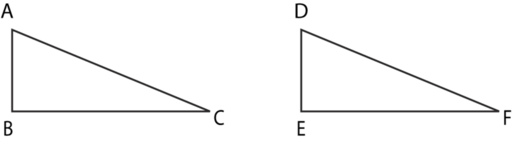
\includegraphics[width=0.45\textwidth]{../images/congruencia02}
        \caption{}
        \label{fig:congruencia01}
    \end{figure}

    \begin{multicols}{2}
        Primero, podemos nombrar los ángulos correspondientes. Los ángulos correspondientes coinciden con ángulos entre los dos triángulos. Los ángulos correspondientes tendrán la misma medida en triángulos congruentes.
        \begin{align*}
            \angle A & \cong \angle D \\
            \angle B & \cong \angle E \\
            \angle C & \cong \angle F \\
        \end{align*}
        Luego, podemos nombrar los lados correspondientes. Los lados correspondientes son lados que coinciden entre los dos triángulos. Tendrán la misma longitud en triángulos congruentes.
        \begin{align*}
            \overline{AB} & \cong \overline{DE} \\
            \overline{AC} & \cong \overline{DF} \\
            \overline{BC} & \cong \overline{EF} \\
        \end{align*}
    \end{multicols}
\end{infocard}